\chapter{THIẾT KẾ HỆ THỐNG}
\ifpdf
    \graphicspath{{Chapter3/Chapter3Figs/PNG/}{Chapter3/Chapter3Figs/PDF/}{Chapter3/Chapter3Figs/}}
\else
    \graphicspath{{Chapter3/Chapter3Figs/EPS/}{Chapter3/Chapter3Figs/}}
\fi

\section{Hướng tiếp cận}
Hình~\ref{fig:wids-traditional} là một giải pháp triển khai hệ thống IDS truyền thống cho mạng không dây. Trong đó:

\begin{itemize}
\item Router: định tuyến và cung cấp kết nối từ mạng nội bộ ra Internet.
\item Switch: được cấu hình kỹ thuật SPAN trên cổng nối ra NIDS. Kỹ thuật này cho phép Switch tự động sao chép các gói tin từ các cổng khác đến cổng giám sát, như vậy toàn bộ lưu thông trong mạng đều được gửi đến NIDS.
\item NIDS: hệ thống phát hiện xâm nhập mạng, giám sát toàn bộ lưu lượng trong mạng có dây và mạng không dây.
\item AP: cung cấp kết nối ra Internet cho các STA.
\item STA: các thiết bị sử dụng mạng không dây.
\end{itemize}

\begin{figure}[H]
    \centering
    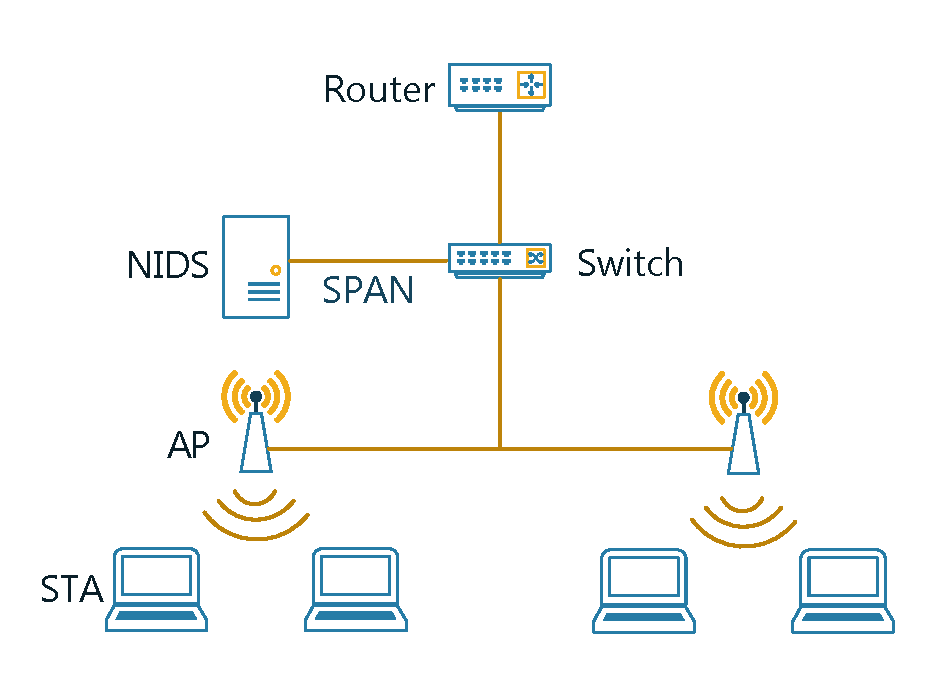
\includegraphics[width=0.8\textwidth]{wids-traditional}
    \caption{
        \label{fig:wids-traditional}
        Giải pháp IDS truyền thống cho mạng không dây}
\end{figure}

Giải pháp này có ưu điểm đó là hệ thống IDS có thể kiểm soát toàn bộ lưu thông vào và ra của mạng không dây. Tuy nhiên, nó không thể kiểm soát liên lạc nội bộ giữa các STA không dây, vì những lưu lượng này không đi qua Switch cũng như NIDS. Giải pháp này cũng không phát hiện được các tấn công từ bên ngoài vào mạng không dây. Ngoài ra, NIDS sẽ phải làm việc với lưu lượng mạng rất lớn, từ cả mạng có dây và mạng không dây, dó đó sẽ ảnh hưởng đến hiệu năng giám sát và phát hiện xâm nhập của NIDS.

Để giám sát các tấn công từ bên ngoài vào mạng không dây, hệ thống sẽ cần thêm các cảm biến không dây (Wireless Sensor). Cảm biến không dây có nhiệm vụ lắng nghe các khung được truyền trong phạm vi thu sóng của nó, sau đó chuyển về máy chủ IDS để xử lý. Như vậy, ngoài các AP để cung cấp kết nối cho các STA, sẽ cần phải có thêm các cảm biến không dây, làm cho chi phí triển khai một hệ thống WIDS tăng lên khá nhiều.

Từ những trở ngại như trên, đồ án xin đưa ra một hướng tiếp cận mới để triển khai một hệ thống WIDS gọi là KMA-WIDS, bằng cách sử dụng các AP như các cảm biến không dây. Các AP này sẽ thu thập các khung quản lý không được mã hóa, để phát hiện các tấn công từ bên ngoài vào mạng không dây. Đồng thời, chúng được cấu hình để tự động sao chép tất cả các gói tin trong mạng không dây và gửi đến cho máy chủ IDS để có thể phát hiện các tấn công bên trong mạng không dây. Hình~\ref{fig:diagram-wids-new} mô tả kiến trúc của hệ thống KMA-WIDS. Các thông tin mà AP thu thập được gửi tới máy chủ IDS, tại đây chúng được xử lý và phát hiện các tấn công, hệ thống sẽ tạo ra các cảnh báo đến giao diện quản trị trên nền tảng web khi phát hiện các tấn công. Ưu điểm của hệ thống này là ứng dụng các phần mềm mã nguồn mở, mang lại một hệ thống WIDS phù hợp về chi phí và hiệu năng.

\begin{figure}[H]
    \centering
    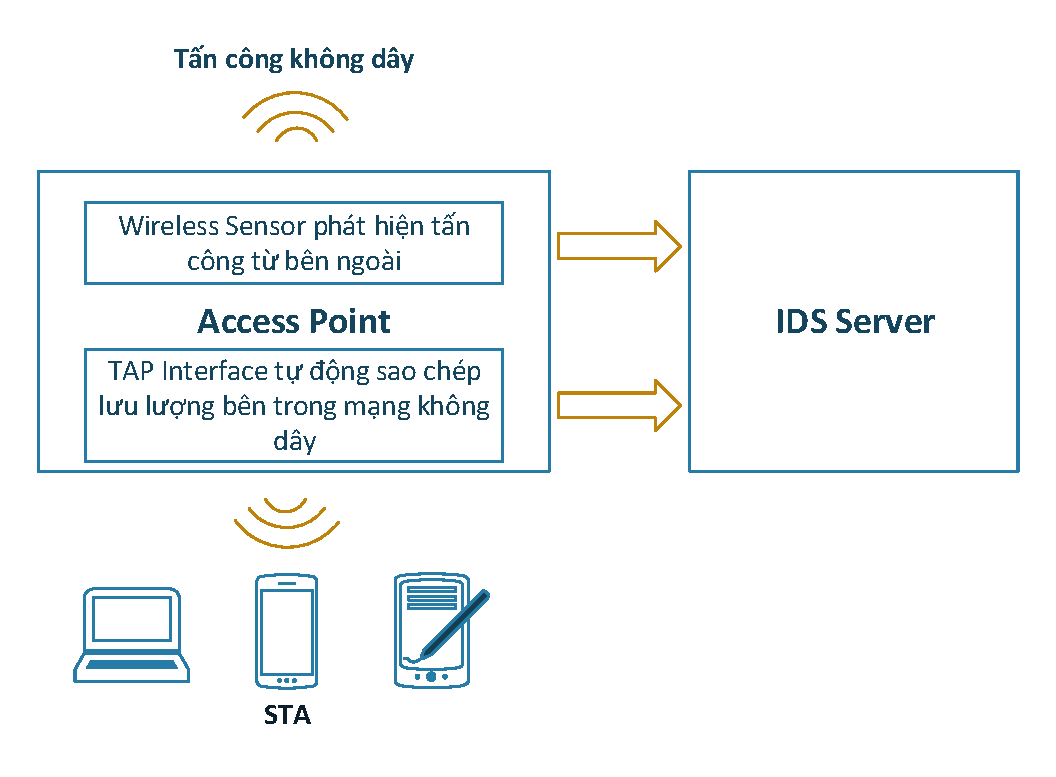
\includegraphics[width=0.85\textwidth]{diagram-wids-new}
    \caption{
        \label{fig:diagram-wids-new}
        Giải pháp KMA-WIDS}
\end{figure}

\section{Các thành phần chính}
Hệ thống WIDS được đề xuất bao gồm hai thiết bị vật lý, một Access Point TP-Link chạy hệ điều hành OpenWrt và một IDS Server dùng máy tính nhúng Raspberry Pi~\cite{rasberry2017raspberry} chạy hệ điều hành Raspbian~\cite{raspberry2017raspbian}. Hình~\ref{fig:diagram-wids-new-components} thể hiện vị trí cụ thể của từng phần mềm trong hệ thống WIDS đề xuất. Cụ thể như sau:

\begin{itemize}
\item OpenWrt: đây sẽ là hệ điều hành mà đồ án chọn để thay thế firmware gốc của AP, như đã trình bày ở chương 2, OpenWrt cung cấp một firmware tối thiểu với khả năng mở rộng cao thông qua việc cài đặt các phần mềm bổ sung.
\item Raspbian: máy tính nhúng Raspberry Pi sẽ được cài đặt Raspbian, một hệ điều hành được tối ưu dựa trên nền tảng Debian, cung cấp một bản Linux rút gọn với đầy đủ chức năng và tương thích với máy tính nhúng Raspberry Pi.

\begin{figure}[H]
    \centering
    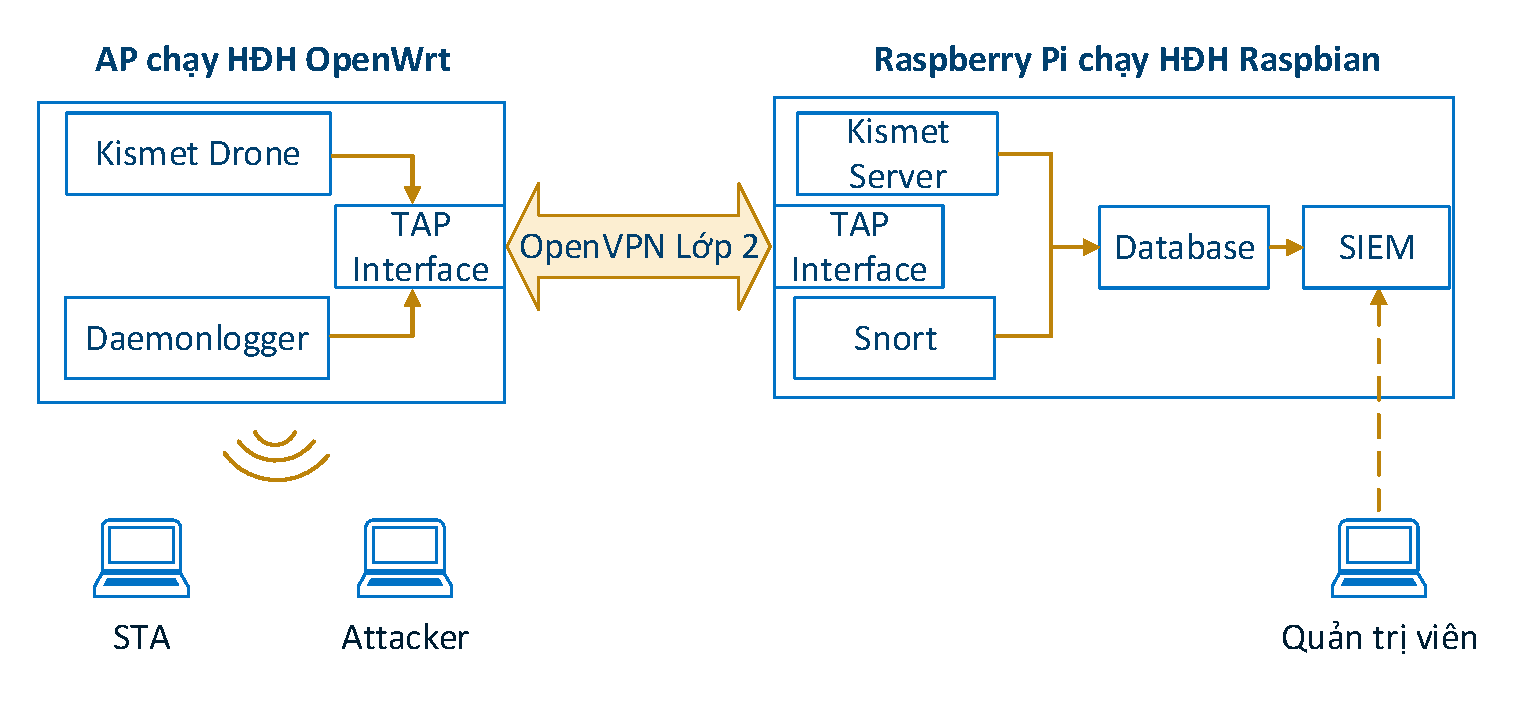
\includegraphics[width=1.0\textwidth]{diagram-wids-new-components}
    \caption{
        \label{fig:diagram-wids-new-components}
        Vị trí các phần mềm trong KMA-WIDS}
\end{figure}

\item Kismet Drone: là gói phần mềm được cài đặt lên OpenWrt để làm nhiệm vụ của một WIDS Sensor, thu thập các khung để hỗ trợ cho việc phát hiện các tấn công từ bên ngoài.
\item Kismet Server: đáp ứng kiến trúc phân tán của Kismet, Kismet Server được cài đặt trên IDS Server để nhận các khung từ Kismet Drone, có nhiệm vụ phát hiện các tấn công từ bên ngoài mạng không dây.
\item Daemonlogger~\cite{martin2008daemonlogger}: là gói phần mềm được cài đặt lên OpenWrt, hoạt động như một "software tap", tự động sao chép các gói tin từ giao diện mạng không dây và gửi về IDS Server qua giao diện mạng ảo TAP interface, hỗ trợ cho việc phát hiện các tấn công bên trong mạng không dây.
\item Snort: gói phần mềm được cài đặt trên IDS Server. Snort sẽ lắng nghe trên TAP interface để nhận các gói tin do Daemonlogger gửi về. Với chế độ hoạt động NIDS, Snort mang lại khả năng phát hiện các tấn công từ bên trong mạng không dây.
\item Database: hệ thống cũng cung cấp khả năng lưu trữ các sự kiện vào cơ sở dữ liệu, thông qua gói phần mềm MySQL~\cite{rasberry2017raspberry} để làm hệ quản trị cơ sở dữ liệu. Ngoài ra, để chuyển đổi định dạng các sự kiện xử lý bằng Kismet Server và Snort thành một định dạng thống nhất, gói phần mềm Barnyard2~\cite{ian2016barnyard2} và Sagan~\cite{quadrant2017sagan} cũng được sử dụng.
\item SIEM (Security Information and Event Management): là một hệ thống quản lý sự kiện an ninh. Trong hệ thống KMA-WIDS, sẽ sử dụng gói phần mềm Snorby~\cite{community2017snorby} được triển khai trên nền Apache HTTP Server~\cite{apache2017apache} để cung cấp một giao diện web quản lý sự kiện an ninh cho hệ thống.
\item OpenVPN~\cite{vpn2017documentation}: gói phần mềm này sẽ được cài đặt và cấu hình ở cả hai thiết bị, nó sẽ tạo ra một kết nối VPN lớp 2 thông qua TAP interface để hỗ trợ cho việc truyền dữ liệu an toàn cho hệ thống WIDS. Đồng thời, còn một số lý do khác mà hệ thống yêu cầu một kết nối VPN lớp 2, sẽ được trình bày ở phần sau.
\item Ngoài ra, hệ thống cũng sử dụng nhiều script để tự động hóa quá trình khởi chạy các phần mềm khi khởi động hệ thống, cũng như một số công cụ và thư viện phụ thuộc để hệ thống có thể hoạt động hoàn chỉnh. 
\end{itemize}

\section{Thiết kế và hoạt động}
\subsection{Thiết bị Access Point}
\subsubsection{Tổng quan}
Để có thể triển khai hệ thống KMA-WIDS, cần sử dụng một thiết bị Access Point có dung lượng bộ nhớ flash trên 8~MB. Vì vậy dòng sản phẩm được đồ án lựa chọn thử nghiệm là TP-Link TL-WR1043ND. Dòng sản phẩm Access Point này có dung lượng bộ nhớ flash từ 8 MB, bộ nhớ RAM từ 32 MB; sử dụng vi mạch không dây Qualcomm Atheros với khả năng hỗ trợ hầu hết các chuẩn WiFi. Nó cũng hỗ trợ 5 cổng Ethernet với tốc độ Gigabit, trong đó 1 cổng dùng để làm kết nối WAN, cung cấp liên lạc ra Internet cho các cổng mạng và kết nối WiFi~\cite{openwrt2017tplink}. 

Đồ án sẽ thực hiện xây dựng một firmware tích hợp và cài đặt thay thế lên Access Point. Firmware OpenWrt là một bản phân phối Linux tối thiểu, do vậy chúng cung cấp khả năng quản lý khá dễ dàng. Sơ đồ kiến trúc bên trong thiết bị được mô tả như Hình~\ref{fig:tp-link-wr1043nd}~\cite{openwrt2017tplink}. Dựa vào sơ đồ, ta có thể thấy OpenWrt ánh xạ các card mạng vật lý thành các giao diện mạng luận lý để quản lý, trong đó:

\begin{itemize}
\item \emph{wlan0}: giao diện mạng đại diện cho card mạng WiFi.
\item \emph{eth1}: giao diện mạng trên Switch để kết nối \emph{wlan0} với Switch. Switch ở đây là một thành phần được tích hợp sẵn bên trong của thiết bị.

\begin{figure}[H]
    \centering
    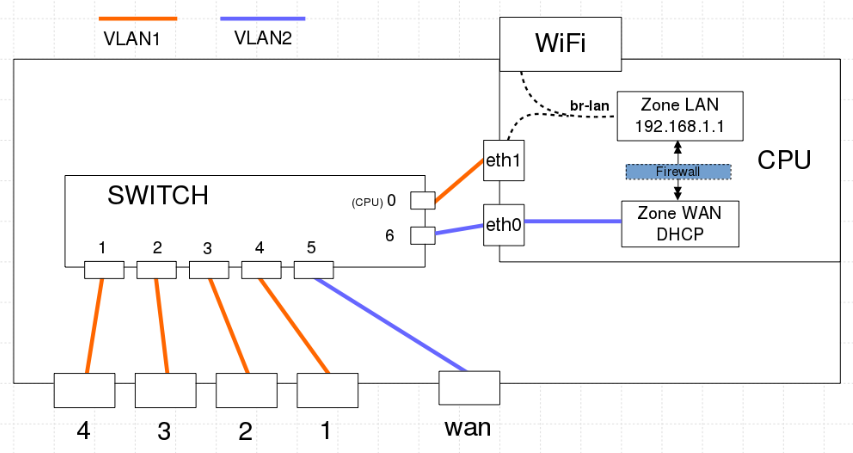
\includegraphics[width=1.0\textwidth]{tp-link-wr1043nd}
    \caption{
        \label{fig:tp-link-wr1043nd}
        Kiến trúc bên trong TP-Link TL-WR1043ND}
\end{figure}

\item \emph{br-lan}: giao diện mạng có nhiệm vụ tạo cầu nối giữa các cổng thuộc VLAN1 trên Switch (\emph{eth1}) với \emph{wlan0} nhằm tạo nên một giao diện mạng chung để kiểm soát truy cập ra Internet, cũng như cho phép các máy tính có dây có thể liên lạc với các STA của mạng WiFi.
\item \emph{eth0}: giao diện mạng trên Switch để cung cấp kết nối ra Internet cho toàn bộ thiết bị, được kiểm soát truy cập thông qua firewall. \emph{eth0} thuộc VLAN2, nên có thể nói nó hoàn toàn độc lập với các cổng thuộc VLAN1 trên Switch.
\item Các cổng trên Switch: được sử dụng để cung cấp kết nối cho các máy tính có dây.
\end{itemize}

\subsubsection{Phương pháp thu thập các khung}
Sau khi thay thế bằng firmware OpenWrt, card mạng không dây của thiết bị TP-Link TL-WR1043ND sử dụng trình điều khiển \emph{mac80211} thông qua gói \emph{kmod-mac80211}~\cite{openwrt2017wiki}. Trình điều khiển \emph{mac80211} cho phép card mạng không dây cùng một lúc có thể hoạt động ở hai chế độ: chế độ Access Point để phát sóng WiFi, chế độ giám sát cho phép lắng nghe và thu thập các khung truyền trong phạm vi thu phát sóng~\cite{steven2015capturing}. Vì đặc điểm này, Kismet Drone khi khởi chạy, sẽ tạo ra một giao diện mạng ảo ở chế độ giám sát là \emph{wlan0mon}, sau đó nó sẽ thu thập các khung thông qua giao diện mạng này, và gửi tới cho Kismet Server trên IDS Server. Giao diện mạng \emph{wlan0} hoạt động ở chế độ Access Point, cung cấp kết nối WiFi cho các STA như bình thường.

\subsubsection{Phương pháp sao chép lưu lượng không dây}
Các cổng trên Switch của Access Point sử dụng chung một giao diện mạng để truy cập ra Internet, đó là \emph{eth1}. Điều này tạo nên một khó khăn khi thực hiện sao chép các lưu lượng không dây từ card mạng không dây, và đẩy đến một cổng cụ thể trên Switch, cổng mà sẽ nối với IDS Server. Khi lưu lượng được gửi đến \emph{eth1}, toàn bộ các cổng trên Switch đều nhận được các lưu lượng này. Các lưu lượng này không yêu cầu được định tuyến hay chuyển mạch, vì vậy việc gửi toàn bộ các cổng sẽ khiến hiệu năng mạng bị ảnh hưởng. Hơn nữa, trong trường hợp này, AP và IDS Server phải kết nối trực tiếp, không thông qua thiết bị nào khác thì mới áp dụng được.

Vấn đề trên đây có hai hướng giải quyết. Cách thứ nhất là thực hiện cấu hình tạo thêm một VLAN3, xóa một cổng cụ thể thuộc VLAN1 và thêm nó vào VLAN3, cổng này sẽ trở thành một cổng quản lý, dùng để kết nối trực tiếp với IDS Server, các lưu lượng trong VLAN3 sẽ độc lập hoàn toàn với hai VLAN còn lại của Switch. Cách thứ hai là thực hiện cấu hình một kết nối VPN lớp 2 giữa Access Point với IDS Server, một kết nối VPN lớp 2 sẽ tạo nên hai giao diện mạng TAP ở hai đầu, giúp cho việc đẩy dữ liệu đến đúng IDS Server thông qua giao diện mạng TAP. Trong cách thứ nhất, có nhược điểm đó là cổng quản lý là một cổng cố định, phải được đánh dấu để tránh nhầm lẫn, bên cạnh đó AP và IDS Server còn phải kết nối trực tiếp với nhau để đảm bảo lưu lượng mạng sao chép đi đúng đến IDS Server. Cách thứ hai mang lại ưu điểm về khả năng linh hoạt và bảo mật, có thể sử dụng bất cứ cổng nào thuộc VLAN1 của thành phần Switch để nối với IDS Server, kết nối VPN lớp 2 sẽ phụ trách phần còn lại, hơn nữa lưu lượng quản lý lúc này được bảo vệ bởi kết nối VPN. Vì những ưu điểm như vậy, đồ án quyết định triển khai theo hướng giải quyết thứ hai, cấu hình một kết nối VPN lớp 2 giữa Access Point và IDS Server.

Một số thiết bị Switch thường có một cổng đặc biệt, gọi là cổng quản lý. Cổng quản lý có thể được cấu hình kỹ thuật SPAN, với tính năng là tự động sao chép tất cả các gói tin lưu thông qua Switch và đẩy về cổng quản lý, phục vụ mục đích giám sát hệ thống mạng, xử lý sự cố. Trong thiết bị Access Point, giao diện mạng không dây không phải là một cổng trên thành phần Switch nên không thể làm được điều này, vì vậy đồ án sẽ sử dụng một phần mềm mã nguồn mở có tên là Daemonlogger, nó có chức năng là sao chép các gói tin từ một giao diện mạng, và đẩy về một giao diện mạng khác. Daemonlogger được viết bởi Martin Roeschi, cũng là tác giả của phần mềm Snort nổi tiếng, thuộc sở hữu của Sourcefire và nay là Cisco~\cite{martin2008daemonlogger}. Daemonlogger là một phần mềm dựa trên thư viện phân tích mạng libpcap, hoạt động của thư viện libpcap được thể hiện trong Hình~\ref{fig:libpcap-works}. Có thể thấy một gói tin nhận được từ bên gửi sẽ được tái tạo hoàn chỉnh ở bên nhận, có nghĩa là sẽ không còn các mã hóa đường truyền. Chính khả năng này làm cho libpcap được sử dụng rộng rãi trong các công cụ phân tích mạng như Snort, tcpdump. Libpcap cũng cho phép sử dụng bộ lọc BPF (Berkeley Packet Filter) để áp dụng những cú pháp lọc lên gói tin thu thập, giúp giảm thiểu lưu lượng cần phân tích.

\begin{figure}[H]
    \centering
    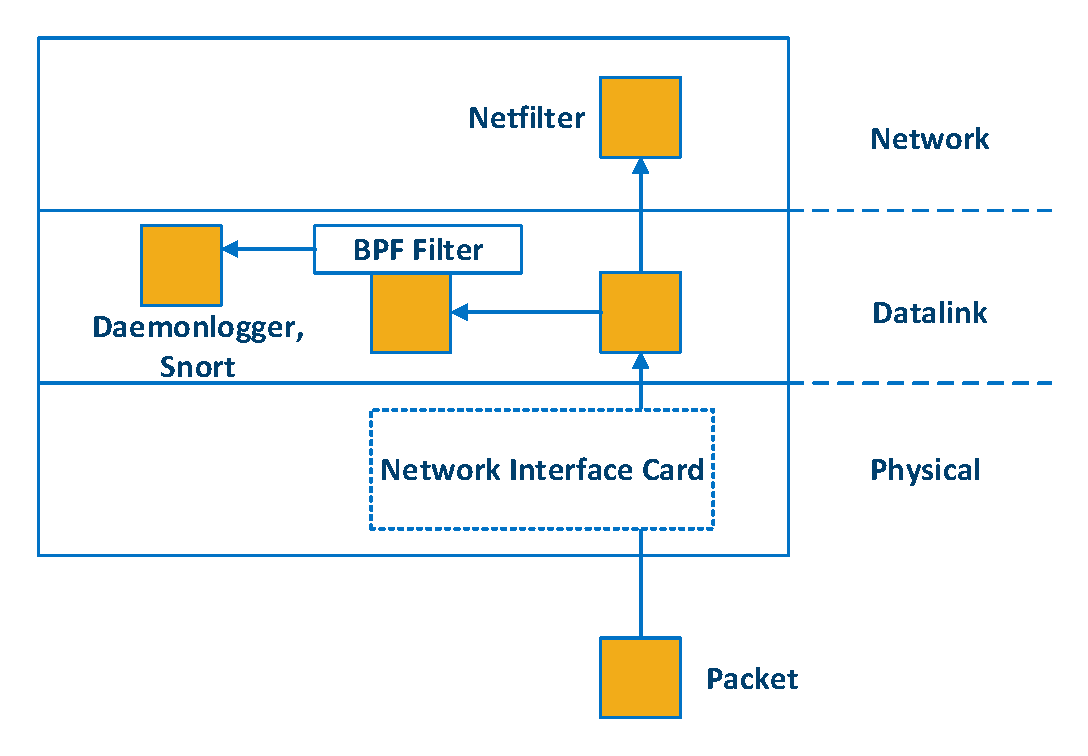
\includegraphics[width=0.9\textwidth]{libpcap-works}
    \caption{
        \label{fig:libpcap-works}
        Hoạt động của libpcap}
\end{figure}

\subsection{Thiết bị máy tính nhúng Raspberry Pi}
\subsubsection{Tổng quan}

Raspberry Pi là một dòng máy tính nhỏ gọn, chỉ bao gồm một bảng mạch có kích thước tương tự như thẻ tín dụng thông thường. 
Hình~\ref{fig:Raspberry-Pi-2-Model-B-1GB} là hình ảnh về các thành phần của một máy tính nhúng Raspberry Pi 2 mẫu B, phiên bản mà đồ án sử dụng. Phiên bản này sử dụng vi xử lý 900~MHz lõi tứ ARM Cortex~-~A7, và bộ nhớ RAM~1GB~\cite{rasberry2017raspberry}. Máy tính nhúng sử dụng hệ điều hành Raspbian, một phiên bản tối ưu dựa trên Debian, cung cấp môi trường Linux chuẩn, đáp ứng nhu cầu sử dụng máy tính cơ bản. Ngoài ra, Raspberry Pi cũng được thiết kế để vận hành liên tục trong thời gian dài, với mức tiêu thụ năng lượng rất thấp~\cite{wikipedia2017raspberry}. Trong đồ án này, máy tính nhúng Raspberry Pi sẽ được cài đặt để làm một IDS Server. Trên đó sẽ cài đặt các phần mềm đảm nhiệm các chức năng cụ thể như mô tả phần mềm ở phần đầu. Sau đây là các luồng xử lý dữ liệu chính mà IDS Server thực hiện.

\begin{figure}[H]
    \centering
    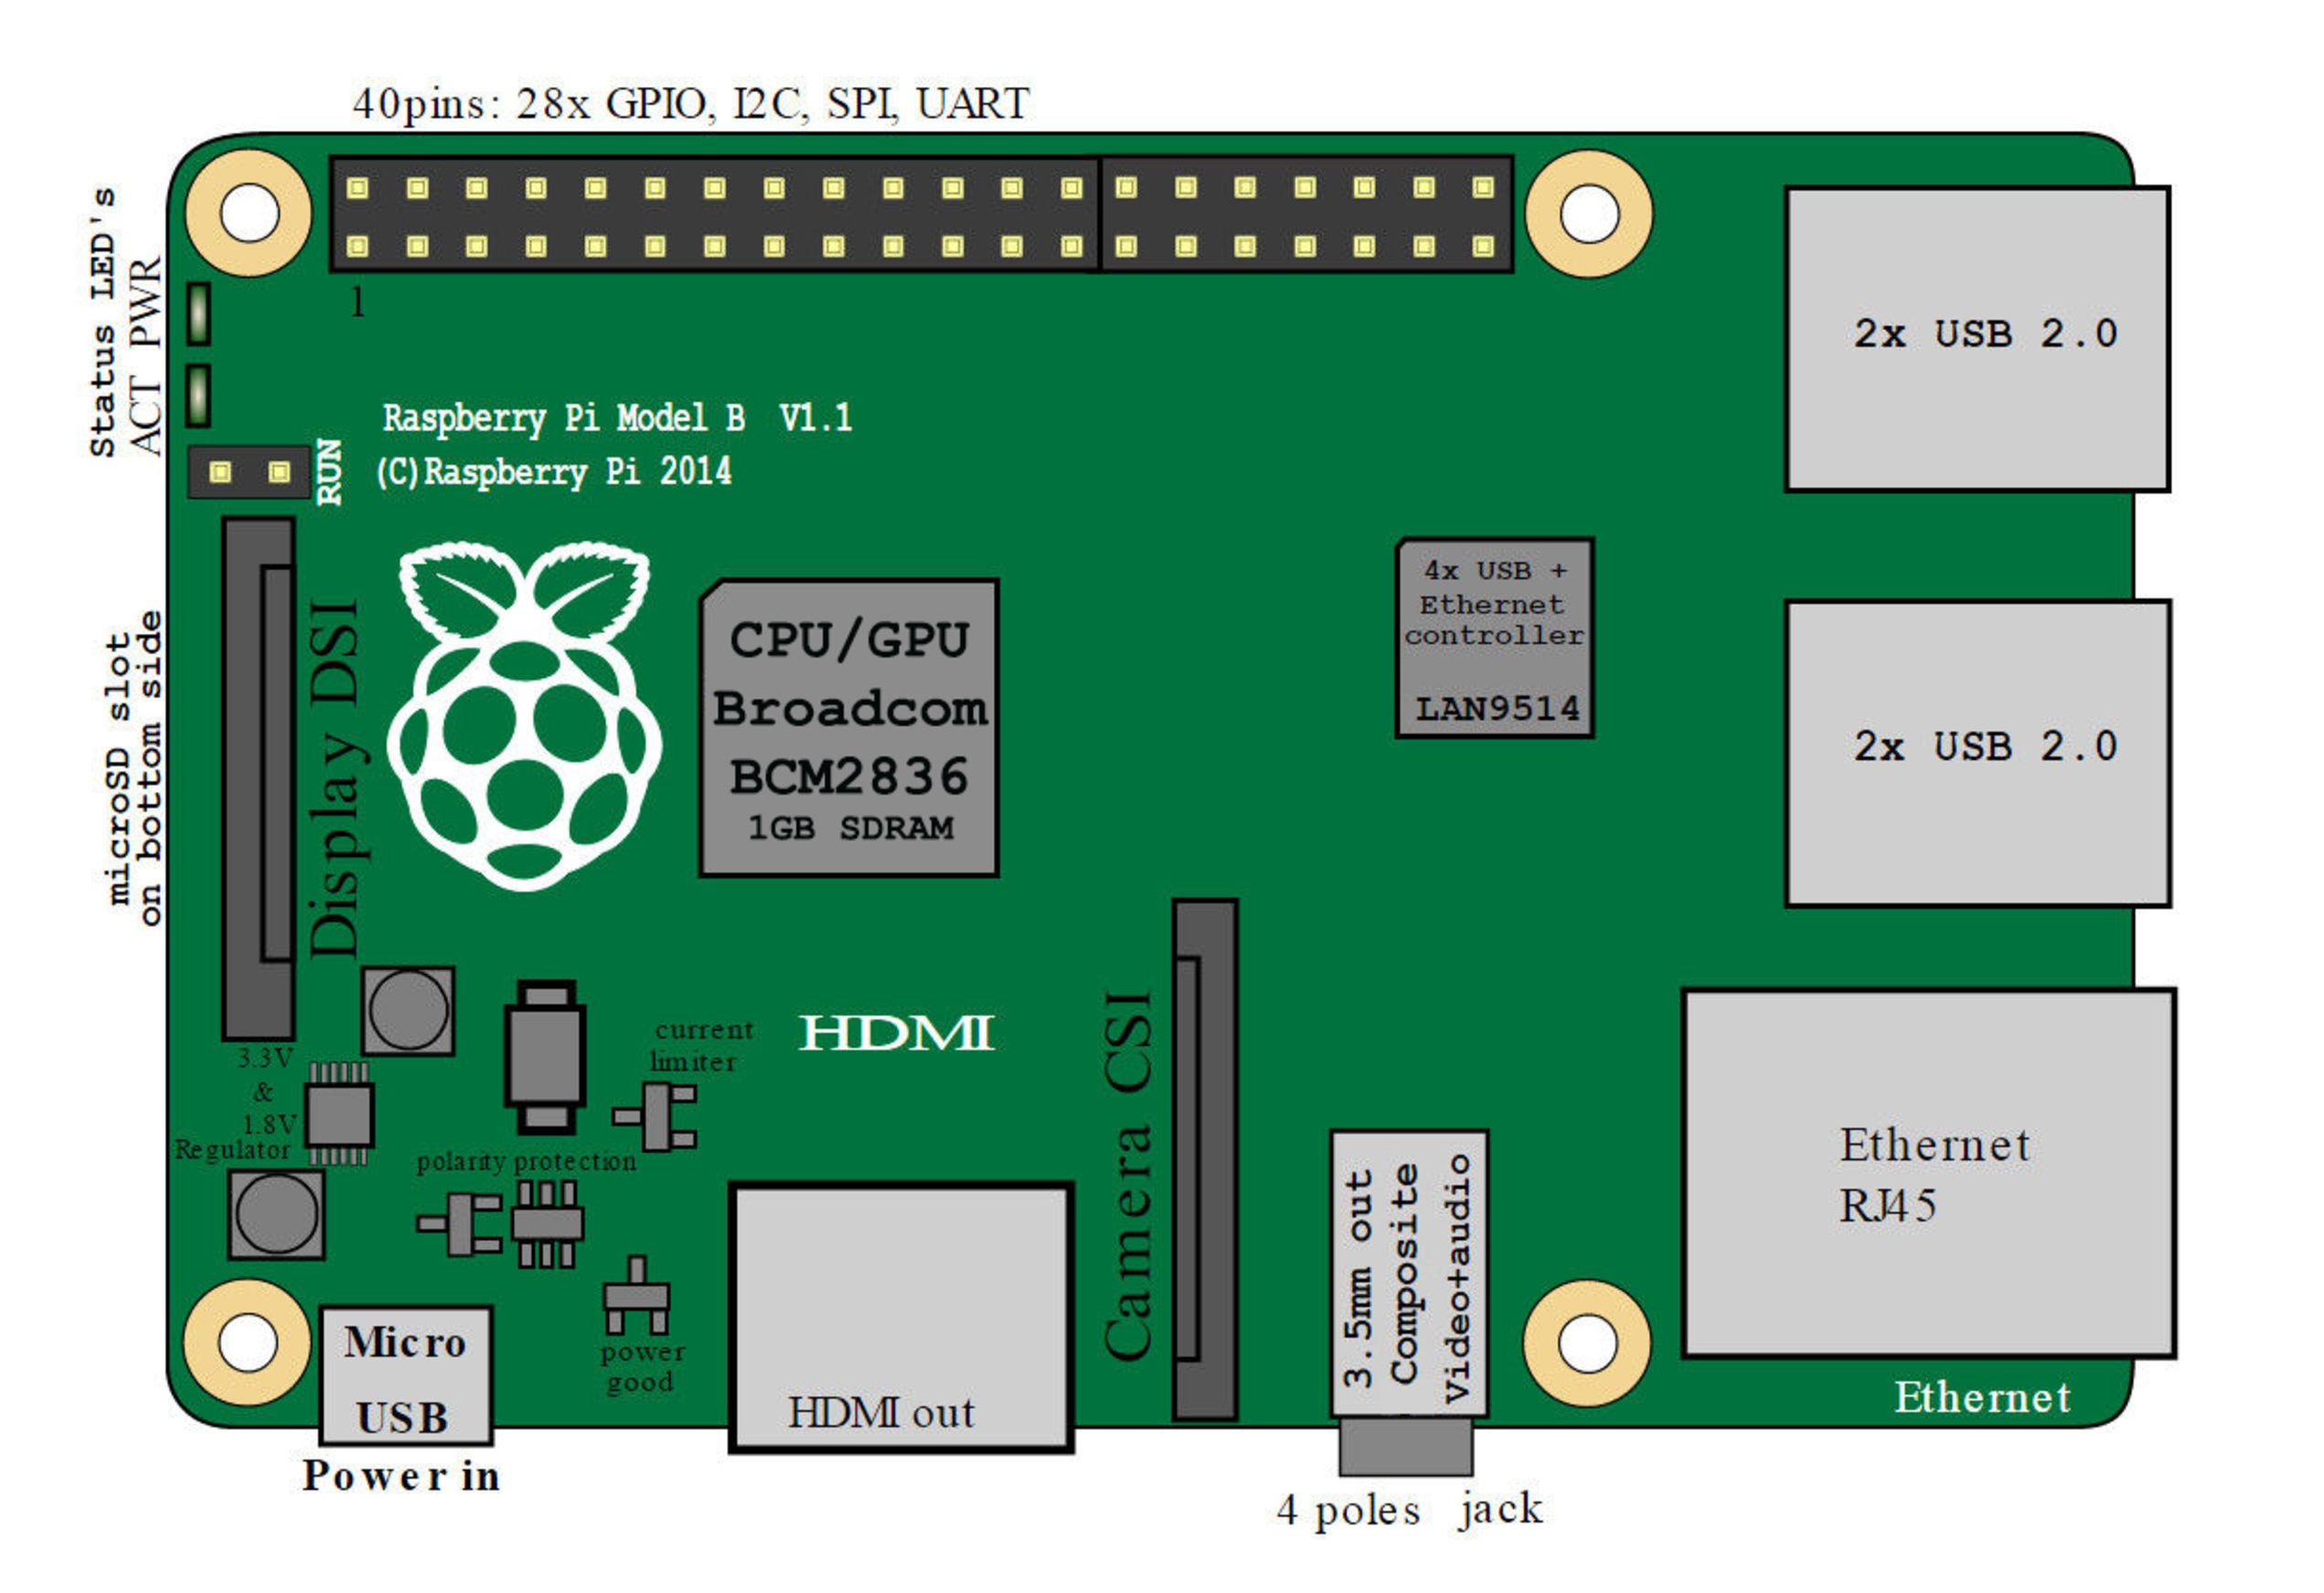
\includegraphics[width=0.9\textwidth]{Raspberry-Pi-2-Model-B-1GB}
    \caption{
        \label{fig:Raspberry-Pi-2-Model-B-1GB}
        Máy tính nhúng Raspberry Pi 2 mẫu B}
\end{figure}

\subsubsection{Luồng xử lý dữ liệu của Kismet}
Luồng xử lý dữ liệu của Kismet được mô tả như Hình~\ref{fig:kismet-workflow}.

\begin{figure}[H]
    \centering
    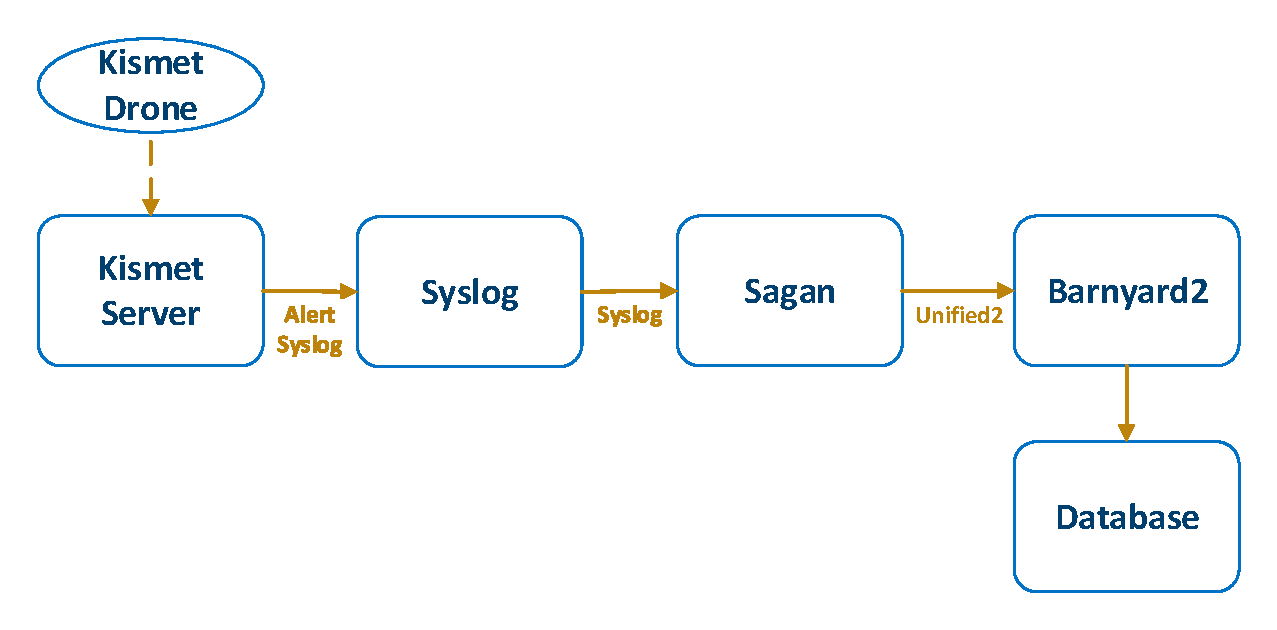
\includegraphics[width=1.0\textwidth]{kismet-workflow}
    \caption{
        \label{fig:kismet-workflow}
        Luồng xử lý dữ liệu của Kismet}
\end{figure}

Sau khi Kismet Drone thu thập các khung quản lý trong phạm vi thu phát sóng, nó sẽ gửi cho Kismet Server. Kismet sử dụng giao thức Kismet Client/Server để liên lạc giữa hai thành phần Kismet Drone và Kismet Server, giao thức này truyền dữ liệu dưới dạng rõ, do vậy thiết lập một kết nối VPN là một việc cần thiết, giúp bảo vệ các dữ liệu này tránh bị những thay đổi không mong muốn. Kismet Server nhận được dữ liệu từ Kismet Drone, sẽ tiến hành xử lý và xuất cảnh báo khi phát hiện tấn công ra các tập tin nhật ký theo mặc định. Vì vậy, đồ án sẽ cài đặt thêm phần mở rộng Alert-Syslog, để Kismet Server có thể gửi các cảnh báo ra cho tiến trình Syslog. Dữ liệu cảnh báo của Kismet và Snort có cú pháp không thống nhất với nhau, trong khi đó, Snort có thể xuất ra định dạng dữ liệu unified2~\cite{snort2017documents}, một định dạng khá phổ biến và được coi như một chuẩn định dạng dữ liệu trong phân tích sự kiện. Do vậy, giải pháp đề ra là cho dữ liệu syslog đi qua phần mềm Sagan, đầu ra của nó sẽ là định dạng unified2 như yêu cầu. Cuối cùng, Barnyard2 sẽ đọc tuần tự các tập tin unified2, để đưa dữ liệu vào cơ sở dữ liệu MySQL một cách hợp lý.

\subsubsection{Luồng xử lý dữ liệu của Snort}
Tiếp đến đồ án sẽ trình bày về luồng xử lý dữ liệu của Snort. Luồng xử lý dữ liệu của Snort được mô tả như Hình~\ref{fig:snort-workflow}.

\begin{figure}[H]
    \centering
    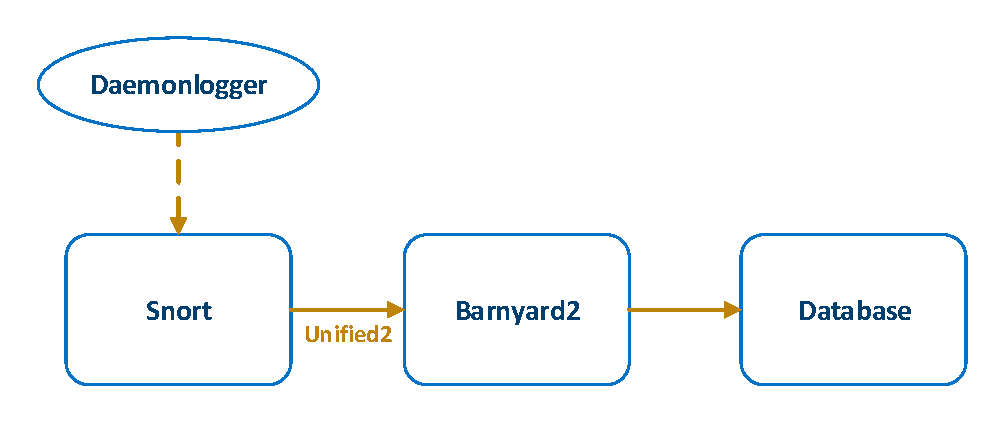
\includegraphics[width=0.9\textwidth]{snort-workflow}
    \caption{
        \label{fig:snort-workflow}
        Luồng xử lý dữ liệu của Snort}
\end{figure}

%\newgeometry{a4paper,left=3.5cm,right=2cm,top=3cm,bottom=3cm}
%\headsep=0pt

Snort cũng như Daemonlogger đều là các phần mềm dựa trên thư viện libpcap. Như đã mô tả về libpcap ở phần trên, Snort sẽ nhận được những gói tin hoàn chỉnh được gửi bởi Daemonlogger thông qua TAP interface. Sau đó, Snort sẽ xử lý những dữ liệu này và xuất các cảnh báo nếu phát hiện các tấn công. Snort hỗ trợ xuất ra định dạng unified2 bằng cách thiết lập tập tin cấu hình cho nó. Dữ liệu unified2 được chuyển đến cho Barnyard2, để phân tích và lưu vào cơ sở dữ liệu.

\subsection{Phần mềm quản lý sự kiện an ninh}
Ngoài ra, để đáp ứng khả năng giám sát và nhận cảnh báo cho người quản trị, hệ thống cũng triển khai một phần mềm quản lý sự kiện an ninh khá đơn giản và hiệu quả, đó là Snorby. Snorby được phát triển trên nền Ruby on Rails, nó sẽ lấy thông tin từ cơ sở dữ liệu MySQL, để đưa ra các thống kê sự kiện và cảnh báo. Snorby cung cấp các chức năng khá trực quan và dễ sử dụng, bao gồm:

\begin{itemize}
\item \emph{Thống kê và báo cáo:} dữ liệu có thể được phân tích và thống kê theo ngày, tuần, tháng, năm. Ngoài ra, nó cũng hỗ trợ xuất báo cáo thành định dạng pdf.
\item \emph{Giám sát và phân loại sự kiện:} các sự kiện được hiển thị theo thời gian thực, người quản trị có thể phân loại những sự kiện này, cũng có thể đưa nó vào hàng đợi để phân loại sau. Snorby cung cấp một số định nghĩa về phân loại có sẵn, hoặc có thể tự định nghĩa theo nhu cầu.
\item \emph{Hiển thị thông tin chi tiết cảnh báo:} Snorby cho phép xem các thông tin chi tiết của một cảnh báo, thậm chí có thể xem chi tiết dữ liệu nguyên thủy bên trong gói tin thu thập được.
\item \emph{Phím tắt:} Snorby sử dụng một hệ thống phím tắt riêng, cho phép người quản trị thay đổi tùy ý. Hệ thống phím tắt này giúp việc phân loại sự kiện hiệu quả và nhanh chóng hơn.
\item \emph{Khả năng mở rộng:} Snorby cũng hỗ trợ một số phần mở rộng từ bên thứ ba.
\end{itemize}

%\restoregeometry

\section{Kết chương}
Như vậy, chương này đồ án đã trình bày về hướng tiếp cận mới của hệ thống KMA-WIDS, cũng như thiết kế tổng quan và chi tiết của nó. Có thể nói, hệ thống WIDS được đề xuất bao gồm đầy đủ các thành phần như một hệ thống IDS tiêu chuẩn như đã trình bày ở chương 2. Chương tiếp theo sẽ trình bày về hiện thực hệ thống, các mô tả cài đặt, giao diện hoạt động, từ đó tiến hành đánh giá về hoạt động của hệ thống.
